% Options for packages loaded elsewhere
\PassOptionsToPackage{unicode}{hyperref}
\PassOptionsToPackage{hyphens}{url}
\PassOptionsToPackage{dvipsnames,svgnames,x11names}{xcolor}
%
\documentclass[
  letterpaper,
  DIV=11,
  numbers=noendperiod]{scrartcl}

\usepackage{amsmath,amssymb}
\usepackage{iftex}
\ifPDFTeX
  \usepackage[T1]{fontenc}
  \usepackage[utf8]{inputenc}
  \usepackage{textcomp} % provide euro and other symbols
\else % if luatex or xetex
  \usepackage{unicode-math}
  \defaultfontfeatures{Scale=MatchLowercase}
  \defaultfontfeatures[\rmfamily]{Ligatures=TeX,Scale=1}
\fi
\usepackage{lmodern}
\ifPDFTeX\else  
    % xetex/luatex font selection
\fi
% Use upquote if available, for straight quotes in verbatim environments
\IfFileExists{upquote.sty}{\usepackage{upquote}}{}
\IfFileExists{microtype.sty}{% use microtype if available
  \usepackage[]{microtype}
  \UseMicrotypeSet[protrusion]{basicmath} % disable protrusion for tt fonts
}{}
\makeatletter
\@ifundefined{KOMAClassName}{% if non-KOMA class
  \IfFileExists{parskip.sty}{%
    \usepackage{parskip}
  }{% else
    \setlength{\parindent}{0pt}
    \setlength{\parskip}{6pt plus 2pt minus 1pt}}
}{% if KOMA class
  \KOMAoptions{parskip=half}}
\makeatother
\usepackage{xcolor}
\setlength{\emergencystretch}{3em} % prevent overfull lines
\setcounter{secnumdepth}{-\maxdimen} % remove section numbering
% Make \paragraph and \subparagraph free-standing
\makeatletter
\ifx\paragraph\undefined\else
  \let\oldparagraph\paragraph
  \renewcommand{\paragraph}{
    \@ifstar
      \xxxParagraphStar
      \xxxParagraphNoStar
  }
  \newcommand{\xxxParagraphStar}[1]{\oldparagraph*{#1}\mbox{}}
  \newcommand{\xxxParagraphNoStar}[1]{\oldparagraph{#1}\mbox{}}
\fi
\ifx\subparagraph\undefined\else
  \let\oldsubparagraph\subparagraph
  \renewcommand{\subparagraph}{
    \@ifstar
      \xxxSubParagraphStar
      \xxxSubParagraphNoStar
  }
  \newcommand{\xxxSubParagraphStar}[1]{\oldsubparagraph*{#1}\mbox{}}
  \newcommand{\xxxSubParagraphNoStar}[1]{\oldsubparagraph{#1}\mbox{}}
\fi
\makeatother

\usepackage{color}
\usepackage{fancyvrb}
\newcommand{\VerbBar}{|}
\newcommand{\VERB}{\Verb[commandchars=\\\{\}]}
\DefineVerbatimEnvironment{Highlighting}{Verbatim}{commandchars=\\\{\}}
% Add ',fontsize=\small' for more characters per line
\usepackage{framed}
\definecolor{shadecolor}{RGB}{241,243,245}
\newenvironment{Shaded}{\begin{snugshade}}{\end{snugshade}}
\newcommand{\AlertTok}[1]{\textcolor[rgb]{0.68,0.00,0.00}{#1}}
\newcommand{\AnnotationTok}[1]{\textcolor[rgb]{0.37,0.37,0.37}{#1}}
\newcommand{\AttributeTok}[1]{\textcolor[rgb]{0.40,0.45,0.13}{#1}}
\newcommand{\BaseNTok}[1]{\textcolor[rgb]{0.68,0.00,0.00}{#1}}
\newcommand{\BuiltInTok}[1]{\textcolor[rgb]{0.00,0.23,0.31}{#1}}
\newcommand{\CharTok}[1]{\textcolor[rgb]{0.13,0.47,0.30}{#1}}
\newcommand{\CommentTok}[1]{\textcolor[rgb]{0.37,0.37,0.37}{#1}}
\newcommand{\CommentVarTok}[1]{\textcolor[rgb]{0.37,0.37,0.37}{\textit{#1}}}
\newcommand{\ConstantTok}[1]{\textcolor[rgb]{0.56,0.35,0.01}{#1}}
\newcommand{\ControlFlowTok}[1]{\textcolor[rgb]{0.00,0.23,0.31}{\textbf{#1}}}
\newcommand{\DataTypeTok}[1]{\textcolor[rgb]{0.68,0.00,0.00}{#1}}
\newcommand{\DecValTok}[1]{\textcolor[rgb]{0.68,0.00,0.00}{#1}}
\newcommand{\DocumentationTok}[1]{\textcolor[rgb]{0.37,0.37,0.37}{\textit{#1}}}
\newcommand{\ErrorTok}[1]{\textcolor[rgb]{0.68,0.00,0.00}{#1}}
\newcommand{\ExtensionTok}[1]{\textcolor[rgb]{0.00,0.23,0.31}{#1}}
\newcommand{\FloatTok}[1]{\textcolor[rgb]{0.68,0.00,0.00}{#1}}
\newcommand{\FunctionTok}[1]{\textcolor[rgb]{0.28,0.35,0.67}{#1}}
\newcommand{\ImportTok}[1]{\textcolor[rgb]{0.00,0.46,0.62}{#1}}
\newcommand{\InformationTok}[1]{\textcolor[rgb]{0.37,0.37,0.37}{#1}}
\newcommand{\KeywordTok}[1]{\textcolor[rgb]{0.00,0.23,0.31}{\textbf{#1}}}
\newcommand{\NormalTok}[1]{\textcolor[rgb]{0.00,0.23,0.31}{#1}}
\newcommand{\OperatorTok}[1]{\textcolor[rgb]{0.37,0.37,0.37}{#1}}
\newcommand{\OtherTok}[1]{\textcolor[rgb]{0.00,0.23,0.31}{#1}}
\newcommand{\PreprocessorTok}[1]{\textcolor[rgb]{0.68,0.00,0.00}{#1}}
\newcommand{\RegionMarkerTok}[1]{\textcolor[rgb]{0.00,0.23,0.31}{#1}}
\newcommand{\SpecialCharTok}[1]{\textcolor[rgb]{0.37,0.37,0.37}{#1}}
\newcommand{\SpecialStringTok}[1]{\textcolor[rgb]{0.13,0.47,0.30}{#1}}
\newcommand{\StringTok}[1]{\textcolor[rgb]{0.13,0.47,0.30}{#1}}
\newcommand{\VariableTok}[1]{\textcolor[rgb]{0.07,0.07,0.07}{#1}}
\newcommand{\VerbatimStringTok}[1]{\textcolor[rgb]{0.13,0.47,0.30}{#1}}
\newcommand{\WarningTok}[1]{\textcolor[rgb]{0.37,0.37,0.37}{\textit{#1}}}

\providecommand{\tightlist}{%
  \setlength{\itemsep}{0pt}\setlength{\parskip}{0pt}}\usepackage{longtable,booktabs,array}
\usepackage{calc} % for calculating minipage widths
% Correct order of tables after \paragraph or \subparagraph
\usepackage{etoolbox}
\makeatletter
\patchcmd\longtable{\par}{\if@noskipsec\mbox{}\fi\par}{}{}
\makeatother
% Allow footnotes in longtable head/foot
\IfFileExists{footnotehyper.sty}{\usepackage{footnotehyper}}{\usepackage{footnote}}
\makesavenoteenv{longtable}
\usepackage{graphicx}
\makeatletter
\def\maxwidth{\ifdim\Gin@nat@width>\linewidth\linewidth\else\Gin@nat@width\fi}
\def\maxheight{\ifdim\Gin@nat@height>\textheight\textheight\else\Gin@nat@height\fi}
\makeatother
% Scale images if necessary, so that they will not overflow the page
% margins by default, and it is still possible to overwrite the defaults
% using explicit options in \includegraphics[width, height, ...]{}
\setkeys{Gin}{width=\maxwidth,height=\maxheight,keepaspectratio}
% Set default figure placement to htbp
\makeatletter
\def\fps@figure{htbp}
\makeatother

\KOMAoption{captions}{tableheading}
\makeatletter
\@ifpackageloaded{tcolorbox}{}{\usepackage[skins,breakable]{tcolorbox}}
\@ifpackageloaded{fontawesome5}{}{\usepackage{fontawesome5}}
\definecolor{quarto-callout-color}{HTML}{909090}
\definecolor{quarto-callout-note-color}{HTML}{0758E5}
\definecolor{quarto-callout-important-color}{HTML}{CC1914}
\definecolor{quarto-callout-warning-color}{HTML}{EB9113}
\definecolor{quarto-callout-tip-color}{HTML}{00A047}
\definecolor{quarto-callout-caution-color}{HTML}{FC5300}
\definecolor{quarto-callout-color-frame}{HTML}{acacac}
\definecolor{quarto-callout-note-color-frame}{HTML}{4582ec}
\definecolor{quarto-callout-important-color-frame}{HTML}{d9534f}
\definecolor{quarto-callout-warning-color-frame}{HTML}{f0ad4e}
\definecolor{quarto-callout-tip-color-frame}{HTML}{02b875}
\definecolor{quarto-callout-caution-color-frame}{HTML}{fd7e14}
\makeatother
\makeatletter
\@ifpackageloaded{caption}{}{\usepackage{caption}}
\AtBeginDocument{%
\ifdefined\contentsname
  \renewcommand*\contentsname{Table of contents}
\else
  \newcommand\contentsname{Table of contents}
\fi
\ifdefined\listfigurename
  \renewcommand*\listfigurename{List of Figures}
\else
  \newcommand\listfigurename{List of Figures}
\fi
\ifdefined\listtablename
  \renewcommand*\listtablename{List of Tables}
\else
  \newcommand\listtablename{List of Tables}
\fi
\ifdefined\figurename
  \renewcommand*\figurename{Figure}
\else
  \newcommand\figurename{Figure}
\fi
\ifdefined\tablename
  \renewcommand*\tablename{Table}
\else
  \newcommand\tablename{Table}
\fi
}
\@ifpackageloaded{float}{}{\usepackage{float}}
\floatstyle{ruled}
\@ifundefined{c@chapter}{\newfloat{codelisting}{h}{lop}}{\newfloat{codelisting}{h}{lop}[chapter]}
\floatname{codelisting}{Listing}
\newcommand*\listoflistings{\listof{codelisting}{List of Listings}}
\makeatother
\makeatletter
\makeatother
\makeatletter
\@ifpackageloaded{caption}{}{\usepackage{caption}}
\@ifpackageloaded{subcaption}{}{\usepackage{subcaption}}
\makeatother
\ifLuaTeX
  \usepackage{selnolig}  % disable illegal ligatures
\fi
\usepackage{bookmark}

\IfFileExists{xurl.sty}{\usepackage{xurl}}{} % add URL line breaks if available
\urlstyle{same} % disable monospaced font for URLs
\hypersetup{
  pdftitle={Exam 2 Review},
  colorlinks=true,
  linkcolor={blue},
  filecolor={Maroon},
  citecolor={Blue},
  urlcolor={Blue},
  pdfcreator={LaTeX via pandoc}}

\title{Exam 2 Review}
\author{}
\date{}

\begin{document}
\maketitle

\begin{tcolorbox}[enhanced jigsaw, colbacktitle=quarto-callout-note-color!10!white, opacitybacktitle=0.6, opacityback=0, colframe=quarto-callout-note-color-frame, colback=white, leftrule=.75mm, arc=.35mm, coltitle=black, breakable, rightrule=.15mm, bottomtitle=1mm, toptitle=1mm, title=\textcolor{quarto-callout-note-color}{\faInfo}\hspace{0.5em}{Note}, titlerule=0mm, bottomrule=.15mm, toprule=.15mm, left=2mm]

Suggested answers can be found
\href{../exam-review/exam-2-review-A.qmd}{here}, but resist the urge to
peek before you go through it yourself.

\end{tcolorbox}

\section{Part 1 - Employment}\label{part-1---employment}

A large university knows that about 70\% of the full-time students are
employed at least 5 hours per week. The members of the Statistics
Department wonder if the same proportion of their students work at least
5 hours per week. They randomly sample 25 majors and find that 15 of the
students (60\%) work 5 or more hours each week.

\subsection{Question 1}\label{question-1}

Describe how you can set up a simulation to estimate the proportion of
statistics majors who work 5 or more hours each week based on this
sample.

\(\vspace{2cm}\)

\subsection{Question 2}\label{question-2}

A bootstrap distribution with 1000 simulations is shown below.
Approximate the bounds of the 95\% confidence interval based on this
distribution.

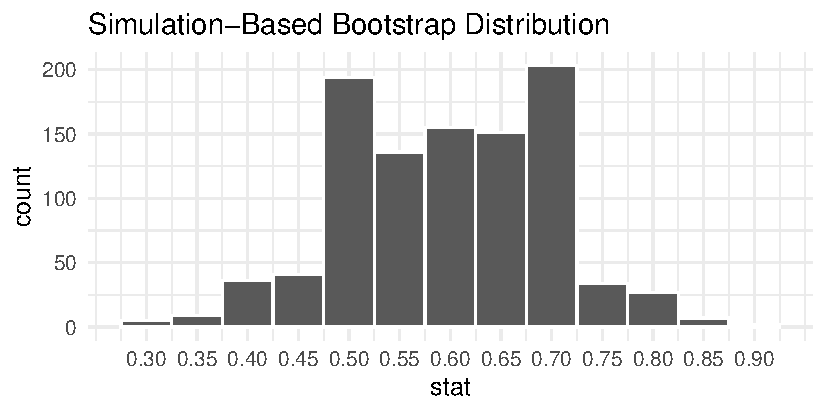
\includegraphics{exam-2-review_files/figure-pdf/unnamed-chunk-2-1.pdf}

\subsection{Question 3}\label{question-3}

Suppose the lower bound of the confidence interval from the previous
question is L and the upper bound is U. Which of the following is
correct?

a. Between L to U of statistics majors work at least 5 hours per week.

b. 95\% of the time the true proportion of statistics majors who work at
least 5 hours per week is between L and U.

c. Between L and U of random samples of 25 statistics majors are
expected to yield confidence intervals that contain the true proportion
of statistics majors who work at least 5 hours per week.

d. 95\% of random samples of 25 statistics majors will yield confidence
intervals between L and U.

e. None of the above.

\newpage{}

\section{Part 2 - Blizzard}\label{part-2---blizzard}

In 2020, employees of Blizzard Entertainment circulated a spreadsheet to
anonymously share salaries and recent pay increases amidst rising
tension in the video game industry over wage disparities and executive
compensation. (Source:
\href{https://www.bloomberg.com/news/articles/2020-08-03/blizzard-workers-share-salaries-in-revolt-over-wage-disparities}{Blizzard
Workers Share Salaries in Revolt Over Pay})

The name of the data frame used for this analysis is
\texttt{blizzard\_salary} and the variables are:

\begin{itemize}
\item
  \texttt{percent\_incr}: Raise given in July 2020, as percent increase
  with values ranging from 1 (1\% increase to 21.5 (21.5\% increase)
\item
  \texttt{salary\_type}: Type of salary, with levels \texttt{Hourly} and
  \texttt{Salaried}
\item
  \texttt{annual\_salary}: Annual salary, in USD, with values ranging
  from \$50,939 to \$216,856.
\item
  \texttt{performance\_rating}: Most recent review performance rating,
  with levels \texttt{Poor}, \texttt{Successful}, \texttt{High}, and
  \texttt{Top}. The \texttt{Poor} level is the lowest rating and the
  \texttt{Top} level is the highest rating.
\end{itemize}

The top ten rows of \texttt{blizzard\_salary} are shown below:

\begin{verbatim}
# A tibble: 409 x 4
   percent_incr salary_type annual_salary performance_rating
          <dbl> <chr>               <dbl> <chr>             
 1          1   Salaried               1  High              
 2          1   Salaried               1  Successful        
 3          1   Salaried               1  High              
 4          1   Hourly             33987. Successful        
 5         NA   Hourly             34798. High              
 6         NA   Hourly             35360  <NA>              
 7         NA   Hourly             37440  <NA>              
 8          0   Hourly             37814. <NA>              
 9          4   Hourly             41101. Top               
10          1.2 Hourly             42328  <NA>              
# i 399 more rows
\end{verbatim}

\subsection{Question 4}\label{question-4}

Next, you fit a model for predicting raises (\texttt{percent\_incr})
from salaries (\texttt{annual\_salary}). We'll call this model
\texttt{raise\_1\_fit}. A tidy output of the model is shown below.

\begin{verbatim}
# A tibble: 2 x 5
  term           estimate  std.error statistic   p.value
  <chr>             <dbl>      <dbl>     <dbl>     <dbl>
1 (Intercept)   1.87      0.432           4.33 0.0000194
2 annual_salary 0.0000155 0.00000452      3.43 0.000669 
\end{verbatim}

Which of the following is the best interpretation of the slope
coefficient?

\begin{enumerate}
\def\labelenumi{\alph{enumi}.}
\tightlist
\item
  For every additional \$1,000 of annual salary, the model predicts the
  raise to be higher, on average, by 1.55\%.
\item
  For every additional \$1,000 of annual salary, the raise goes up by
  0.0155\%.
\item
  For every additional \$1,000 of annual salary, the model predicts the
  raise to be higher, on average, by 0.0155\%.
\item
  For every additional \$1,000 of annual salary, the model predicts the
  raise to be higher, on average, by 1.87\%.
\end{enumerate}

\subsection{Question 5}\label{question-5}

You then fit a model for predicting raises (\texttt{percent\_incr}) from
salaries (\texttt{annual\_salary}) and performance ratings
(\texttt{performance\_rating}). We'll call this model
\texttt{raise\_2\_fit}. Which of the following is definitely true based
on the information you have so far?

\begin{enumerate}
\def\labelenumi{\alph{enumi}.}
\tightlist
\item
  Intercept of \texttt{raise\_2\_fit} is higher than intercept of
  \texttt{raise\_1\_fit}.
\item
  Slope of \texttt{raise\_2\_fit} is higher than RMSE of
  \texttt{raise\_1\_fit}.
\item
  Adjusted \(R^2\) of \texttt{raise\_2\_fit} is higher than adjusted
  \(R^2\) of \texttt{raise\_1\_fit}.
\item
  \(R^2\) of \texttt{raise\_2\_fit} is higher \(R^2\) of
  \texttt{raise\_1\_fit}.
\end{enumerate}

\subsection{Question 6}\label{question-6}

The tidy model output for the \texttt{raise\_2\_fit} model you fit is
shown below.

\begin{verbatim}
# A tibble: 5 x 5
  term                            estimate  std.error statistic  p.value
  <chr>                              <dbl>      <dbl>     <dbl>    <dbl>
1 (Intercept)                   3.55       0.508           6.99 1.99e-11
2 annual_salary                 0.00000989 0.00000436      2.27 2.42e- 2
3 performance_ratingPoor       -4.06       1.42           -2.86 4.58e- 3
4 performance_ratingSuccessful -2.40       0.397          -6.05 4.68e- 9
5 performance_ratingTop         2.99       0.715           4.18 3.92e- 5
\end{verbatim}

When your teammate sees this model output, they remark ``The coefficient
for \texttt{performance\_ratingSuccessful} is negative, that's weird. I
guess it means that people who get successful performance ratings get
lower raises.'' How would you respond to your teammate?

\(\vspace{2cm}\)

\subsection{Question 7}\label{question-7}

Ultimately, your teammate decides they don't like the negative slope
coefficients in the model output you created (not that there's anything
wrong with negative slope coefficients!), does something else, and comes
up with the following model output.

\begin{verbatim}
# A tibble: 5 x 5
  term                            estimate  std.error statistic    p.value
  <chr>                              <dbl>      <dbl>     <dbl>      <dbl>
1 (Intercept)                  -0.511      1.47          -0.347 0.729     
2 annual_salary                 0.00000989 0.00000436     2.27  0.0242    
3 performance_ratingSuccessful  1.66       1.42           1.17  0.242     
4 performance_ratingHigh        4.06       1.42           2.86  0.00458   
5 performance_ratingTop         7.05       1.53           4.60  0.00000644
\end{verbatim}

Unfortunately they didn't write their code in a Quarto document, instead
just wrote some code in the Console and then lost track of their work.
They remember using the \texttt{fct\_relevel()} function and doing
something like the following:

\begin{Shaded}
\begin{Highlighting}[]
\NormalTok{blizzard\_salary }\OtherTok{\textless{}{-}}\NormalTok{ blizzard\_salary }\SpecialCharTok{|\textgreater{}}
  \FunctionTok{mutate}\NormalTok{(}\AttributeTok{performance\_rating =} \FunctionTok{fct\_relevel}\NormalTok{(performance\_rating, \_\_\_))}
\end{Highlighting}
\end{Shaded}

What should they put in the blanks to get the same model output as
above?

\begin{enumerate}
\def\labelenumi{\alph{enumi}.}
\tightlist
\item
  ``Poor'', ``Successful'', ``High'', ``Top''
\item
  ``Successful'', ``High'', ``Top''
\item
  ``Top'', ``High'', ``Successful'', ``Poor''
\item
  Poor, Successful, High, Top
\end{enumerate}

\subsection{Question 8}\label{question-8}

Suppose we fit a model to predict \texttt{percent\_incr} from
\texttt{annual\_salary} and \texttt{salary\_type}. A tidy output of the
model is shown below.

\begin{verbatim}
# A tibble: 3 x 5
  term                 estimate  std.error statistic p.value
  <chr>                   <dbl>      <dbl>     <dbl>   <dbl>
1 (Intercept)         1.24      0.570           2.18 0.0300 
2 annual_salary       0.0000137 0.00000464      2.96 0.00329
3 salary_typeSalaried 0.913     0.544           1.68 0.0938 
\end{verbatim}

Which of the following visualizations represent this model? Explain your
reasoning.

\begin{figure}

\begin{minipage}{0.50\linewidth}

\centering{

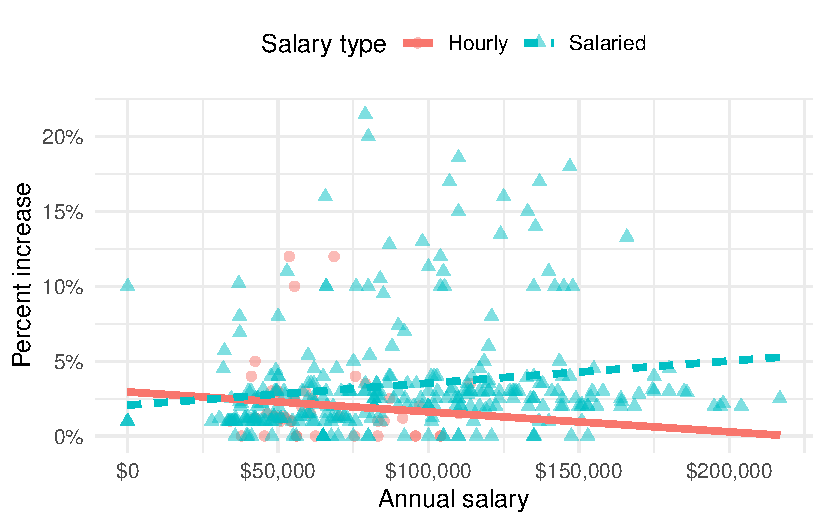
\includegraphics{exam-2-review_files/figure-pdf/fig-raise-salary-type-1.pdf}

}

\subcaption{\label{fig-raise-salary-type-1}Option 1}

\end{minipage}%
%
\begin{minipage}{0.50\linewidth}

\centering{

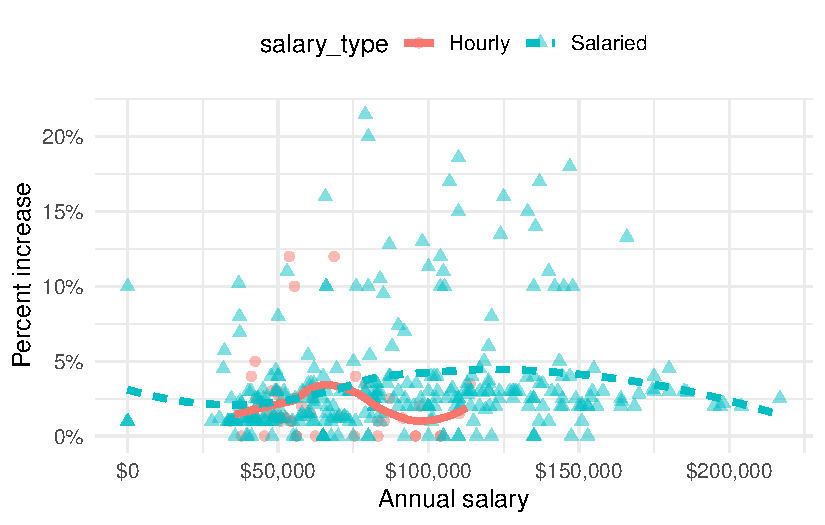
\includegraphics{exam-2-review_files/figure-pdf/fig-raise-salary-type-2.pdf}

}

\subcaption{\label{fig-raise-salary-type-2}Option 2}

\end{minipage}%
\newline
\begin{minipage}{0.50\linewidth}

\centering{

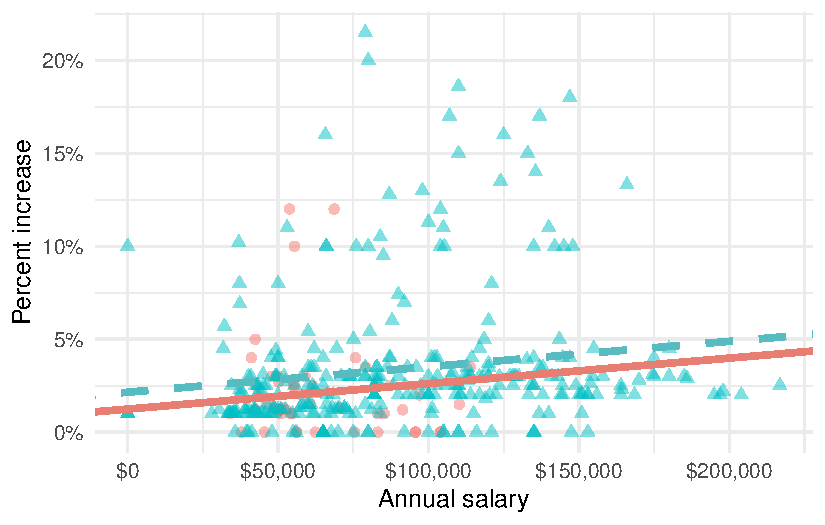
\includegraphics{exam-2-review_files/figure-pdf/fig-raise-salary-type-3.pdf}

}

\subcaption{\label{fig-raise-salary-type-3}Option 3}

\end{minipage}%
%
\begin{minipage}{0.50\linewidth}

\centering{

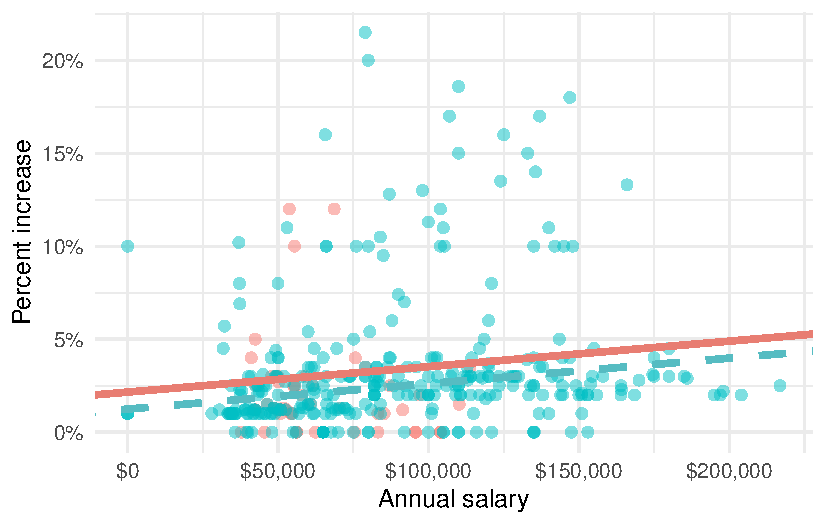
\includegraphics{exam-2-review_files/figure-pdf/fig-raise-salary-type-4.pdf}

}

\subcaption{\label{fig-raise-salary-type-4}Option 4}

\end{minipage}%

\caption{\label{fig-raise-salary-type}Visualizations of the relationship
between percent increase, annual salary, and salary type}

\end{figure}%

\newpage{}

\subsection{Question 9}\label{question-9}

Define the term parsimonious model.

\(\vspace{2cm}\)

\newpage{}

\subsection{Question 10}\label{question-10}

Suppose you now fit a model to predict the natural log of percent
increase, \texttt{log(percent\_incr)}, from performance rating. The
model is called \texttt{raise\_4\_fit}.

You're provided the following:

\begin{Shaded}
\begin{Highlighting}[]
\FunctionTok{tidy}\NormalTok{(raise\_4\_fit) }\SpecialCharTok{|\textgreater{}}
  \FunctionTok{select}\NormalTok{(term, estimate) }\SpecialCharTok{|\textgreater{}}
  \FunctionTok{mutate}\NormalTok{(}\AttributeTok{exp\_estimate =} \FunctionTok{exp}\NormalTok{(estimate))}
\end{Highlighting}
\end{Shaded}

\begin{verbatim}
# A tibble: 4 x 3
  term                         estimate exp_estimate
  <chr>                           <dbl>        <dbl>
1 (Intercept)                     -7.15     0.000786
2 performance_ratingSuccessful     6.93  1025.      
3 performance_ratingHigh           8.17  3534.      
4 performance_ratingTop            8.91  7438.      
\end{verbatim}

Based on this, which of the following is true?

a. The model predicts that the percentage increase employees with
Successful performance get, on average, is higher by 10.25\% compared to
the employees with Poor performance rating.

b. The model predicts that the percentage increase employees with
Successful performance get, on average, is higher by 6.93\% compared to
the employees with Poor performance rating.

c. The model predicts that the percentage increase employees with
Successful performance get, on average, is higher by a factor of 1025
compared to the employees with Poor performance rating.

d. The model predicts that the percentage increase employees with
Successful performance get, on average, is higher by a factor of 6.93
compared to the employees with Poor performance rating.

\section{Part 3 - Miscellaneous}\label{part-3---miscellaneous}

\subsection{Question 11}\label{question-11}

Which of the following is the definiton of a regression model? Select
all that apply.

a. \(\hat{y} = \beta_0 + \beta_1 X_1\)

b. \(y = \beta_0 + \beta_1 X_1\)

c. \(\hat{y} = \beta_0 + \beta_1 X_1 + \epsilon\)

d. \(y = \beta_0 + \beta_1 X_1 + \epsilon\)

\subsection{Question 12}\label{question-12}

\textbf{Choose the best answer.}

A survey based on a random sample of 2,045 American teenagers found that
a 95\% confidence interval for the mean number of texts sent per month
was (1450, 1550). A valid interpretation of this interval is

\begin{enumerate}
\def\labelenumi{\alph{enumi}.}
\tightlist
\item
  95\% of all teens who text send between 1450 and 1550 text messages
  per month.
\item
  If a new survey with the same sample size were to be taken, there is a
  95\% chance that the mean number of texts in the sample would be
  between 1450 and 1550.
\item
  We are 95\% confident that the mean number of texts per month of all
  American teens is between 1450 and 1550.
\item
  We are 95\% confident that, were we to repeat this survey, the mean
  number of texts per month of those taking part in the survey would be
  between 1450 and 1550.
\end{enumerate}

\newpage{}

\subsection{Bonus}\label{bonus}

Pick a concept we introduced in class so far that you've been struggling
with and explain it in your own words.



\end{document}
